\chapter{Fundamentação Teórica}

Este capítulo apresenta os principais conceitos, práticas e tecnologias que sustentam a construção de sistemas distribuídos resilientes baseados em microsserviços. São abordadas as diferentes abordagens arquiteturais, bem como os mecanismos e ferramentas essenciais para garantir a escalabilidade, a robustez e a confiabilidade dessas aplicações. Essa fundamentação destaca as relações de dependência entre essas tecnologias e os trade-offs envolvidos em sua aplicação, estabelecendo assim a base conceitual e técnica para o desenvolvimento e validação do modelo de maturidade proposto.

\section{Arquitetura de Software}

A arquitetura de software ocupa um papel estratégico na engenharia de software, pois influencia diretamente decisões de design, desempenho, manutenibilidade e escalabilidade ao longo do ciclo de vida de um sistema. De acordo com a norma ANSI/IEEE 1471-2000 \citep{Electrical2007}, a arquitetura de um sistema é definida como sua organização fundamental, incluindo componentes, interações entre eles e princípios que orientam seu projeto e evolução. Essa compreensão vai além de aspectos técnicos, pois a arquitetura também reflete fatores organizacionais e práticas de desenvolvimento.

\subsection{Arquitetura Monolítica}

Historicamente, a Arquitetura Monolítica surgiu como o modelo dominante para o desenvolvimento de aplicações. Nesse modelo, o aplicativo é construído como um único projeto, utilizando um único sistema de compilação e resultando em um binário executável que reúne diversos módulos voltados a recursos técnicos ou de negócios \citep{mendes2021arquitetura}. Essa abordagem se consolidou pela sua simplicidade inicial: ao manter todas as funcionalidades em um único processo, as equipes têm menos preocupações com a comunicação entre módulos e podem focar na entrega de funcionalidades de forma rápida \citep{PereiraDiniz2022}.

A Figura~\ref{fig:monolito-diagrama} ilustra como essa arquitetura agrupa a interface do usuário, o núcleo da aplicação e o banco de dados em um único bloco coeso. Esse modelo reduz a complexidade inicial de integração e facilita o monitoramento, já que todas as operações são executadas dentro do mesmo ambiente \citep{Salaheddin2022}.

\begin{figure}[H]
\centering
\includegraphics[width=0.3\linewidth]{imagens/monolito-diagrama.png}
\caption{Diagrama representativo de uma arquitetura monolítica.}
\label{fig:monolito-diagrama}
\end{figure}

Contudo, segundo \citep{fowler2015monolithfirst}, embora a arquitetura monolítica seja um excelente ponto de partida, ela apresenta desafios à medida que o sistema cresce e se torna mais complexo. Problemas de escalabilidade e pontos únicos de falha surgem quando um único binário precisa atender a múltiplas demandas ao mesmo tempo. Isso gera a necessidade de soluções mais flexíveis e adaptáveis para lidar com a evolução constante das aplicações e das demandas do mercado.

\subsection{Arquitetura de Microsserviços}

É nesse cenário de evolução e necessidade de adaptação que a Arquitetura de Microsserviços ganha destaque. Essa abordagem visa superar as limitações do monólito, dividindo a aplicação em pequenos serviços autônomos e independentes, cada um responsável por uma funcionalidade específica e executando seu próprio processo \citep{martinfowler2014microservices}. Esses microsserviços se comunicam entre si por meio de APIs (Interfaces de Programação de Aplicações) baseadas em HTTP (Hypertext Transfer Protocol), formando um ecossistema distribuído e colaborativo.

A Figura~\ref{fig:diagrama-microsservicos} ilustra essa transição arquitetural: cada retângulo representa um microsserviço, com seu próprio banco de dados isolado, mostrando como a separação de responsabilidades facilita o desenvolvimento e a manutenção. A interface do usuário atua como ponto de entrada, direcionando requisições aos microsserviços especializados.

\begin{figure}[H]
\centering
\includegraphics[width=0.7\linewidth]{imagens/microsservico-diagrama.png}
\caption{Diagrama de microsserviços com interface, serviços e bancos de dados independentes.}
\label{fig:diagrama-microsservicos}
\end{figure}

Essa descentralização traz ganhos significativos: cada serviço pode ser escalado horizontalmente de forma independente, adaptando-se às demandas específicas de carga sem impactar outros serviços. Isso aumenta a flexibilidade e a resiliência do sistema como um todo. No entanto, também introduz novos desafios, como a necessidade de ferramentas de observabilidade para monitorar métricas, logs e verificações de saúde de cada serviço \citep{Newman:15:MS}. Além disso, migrar de um sistema monolítico para uma arquitetura distribuída exige estratégias cuidadosas de orquestração e coreografia, garantindo que os serviços colaborem de forma eficiente e confiável \citep{baskarada2018}.

Assim, a passagem de uma arquitetura monolítica para microsserviços não é apenas uma mudança técnica, mas também um reflexo de como as organizações se adaptam à complexidade e à necessidade de resiliência em sistemas distribuídos modernos. Esse movimento de evolução arquitetural fundamenta o modelo de maturidade proposto neste trabalho, que visa apoiar organizações na transição para ambientes mais flexíveis e robustos, aproveitando os benefícios dos microsserviços sem ignorar os desafios operacionais que acompanham essa jornada.

\subsection{Arquitetura Orientada a Eventos}

A necessidade de lidar com cenários de alta demanda e picos de acesso, bem como de garantir maior adaptabilidade, impulsionou o surgimento de abordagens que complementam a arquitetura de microsserviços. Nesse contexto, a Arquitetura Orientada a Eventos (EDA, do inglês \textit{Event-Driven Architecture}) desponta como uma solução poderosa para desacoplar componentes e permitir que eles reajam a mudanças e estímulos de forma assíncrona \citep{Michelson2006}.

Na EDA, eventos representam ocorrências significativas no domínio do negócio ou do sistema, indicando mudanças de estado, anomalias ou oportunidades. Esses eventos são capturados e processados por componentes modulares e independentes, que executam tarefas específicas de maneira desacoplada e assíncrona. Essa característica fortalece a escalabilidade e a adaptabilidade do sistema, pois cada componente atua de forma isolada, sem precisar conhecer os demais ou saber quem irá reagir aos eventos gerados \citep{10.5555/2904417, lazzari2021}.

A Figura~\ref{fig:diagrama-microsservicos} — que ilustra a arquitetura de microsserviços — ajuda a entender como a EDA complementa essa abordagem. Enquanto os microsserviços são responsáveis por funcionalidades bem definidas, a EDA permite que esses serviços interajam de forma reativa, respondendo a eventos que circulam entre eles. Esse modelo reduz ainda mais o acoplamento e aumenta a flexibilidade operacional, criando fluxos de processamento mais dinâmicos e resilientes.

A EDA pode ser implementada seguindo duas topologias principais:

\begin{itemize}
    \item \textbf{Mediator Topology:} utiliza um mediador central para orquestrar eventos complexos com múltiplos passos\footnote{O termo "Mediator" também é conhecido como um padrão de projeto do GoF (Gang of Four), descrito no livro \textit{Design Patterns: Elements of Reusable Object-Oriented Software} (1994). Embora compartilhem o princípio de centralizar a comunicação para evitar acoplamento direto, no contexto da EDA o Mediator atua em nível arquitetural, coordenando eventos em sistemas distribuídos, enquanto no padrão GoF atua em nível de objetos dentro de um único processo.}. É ideal para fluxos que exigem coordenação explícita \citep{10.5555/2904417}.

    
    \item \textbf{Broker Topology:} dispensa o mediador e conecta processadores de eventos diretamente por meio de um \textit{broker}. Cada processador atua de forma autônoma, consumindo eventos, executando lógicas específicas e publicando novos eventos, o que favorece a escalabilidade e a flexibilidade \citep{10.5555/2904417}. Um exemplo clássico é o registro de estatísticas e recomendações em plataformas de streaming de vídeo, onde diversos componentes atuam simultaneamente de maneira descentralizada.
\end{itemize}

Ambas as topologias eliminam dependências diretas entre os componentes, alinhando-se ao princípio de que “emissores não precisam conhecer os receptores” \citep{lazzari2021}. Essa separação entre quem emite e quem consome eventos fortalece a flexibilidade e a adaptabilidade da arquitetura, pois cada componente ou serviço pode evoluir, ser substituído ou escalado de maneira independente, sem impacto direto nos demais.

Além de facilitar a manutenção e a evolução dos sistemas, esse baixo acoplamento reduz os pontos de falha e aumenta a resiliência do ecossistema como um todo. Cada serviço ou processador de eventos tem a liberdade de reagir de acordo com sua lógica de negócios e com a disponibilidade de recursos, sem depender de uma sequência rígida de chamadas ou de um fluxo de controle centralizado. Assim, mesmo em situações adversas ou de alta demanda, os componentes continuam a operar de forma autônoma e coordenada, garantindo a continuidade dos serviços e a robustez do sistema.

Essa capacidade de resposta independente e dinâmica, proporcionada pela Arquitetura Orientada a Eventos, torna-se especialmente valiosa em ambientes distribuídos e complexos, onde a previsibilidade é limitada e a adaptabilidade é essencial para lidar com falhas e variações na carga de trabalho.

\section{Escalabilidade Horizontal e Vertical}
A necessidade de manter um desempenho estável em ambientes distribuídos exige que sistemas modernos incorporem mecanismos de escalabilidade adequados. Essa escalabilidade pode ser classificada em duas formas principais: horizontal e vertical. 

A primeira, conhecida também como \textit{scaling out}, consiste em adicionar novas instâncias ao sistema, distribuindo a carga entre diversos recursos computacionais. Já a escalabilidade vertical — ou \textit{scaling up} — está relacionada ao aumento da capacidade de uma única instância, adicionando mais poder de CPU, memória ou armazenamento. Ambas as abordagens visam melhorar o desempenho e a capacidade de resposta dos sistemas, sendo a escolha entre elas dependente das características da aplicação e do ambiente de implantação \citep{9717259}.

\section{Load Balancer}

Conforme as aplicações evoluíram de sistemas monolíticos para microsserviços e arquiteturas orientadas a eventos, a necessidade de lidar com grandes volumes de requisições e garantir escalabilidade e desempenho contínuos se tornou ainda mais crítica. Nesse cenário, o balanceamento de carga surge como uma técnica fundamental para manter a disponibilidade e a confiabilidade dos sistemas distribuídos.

O balanceamento de carga consiste em distribuir de forma equilibrada o tráfego de requisições entre diferentes servidores, evitando que apenas um nó seja sobrecarregado enquanto outros permanecem subutilizados \citep{mohapatra2013}. Esse processo não apenas otimiza o uso de recursos e reduz o tempo de resposta, mas também reforça a resiliência geral da aplicação, permitindo que ela suporte picos de acesso e situações de alta demanda sem comprometer a experiência do usuário.

Na prática, o balanceador de carga costuma ser posicionado entre os usuários e o conjunto de servidores que executam as aplicações. Embora essa não seja uma configuração obrigatória, ela é amplamente adotada porque permite que todo o tráfego seja gerenciado de maneira centralizada e transparente, sem que o usuário perceba as complexidades envolvidas \citep{kumar2016}. Atuando como uma ponte de intermediação, o balanceador intercepta as requisições e as distribui para os servidores disponíveis, ajustando-se dinamicamente à carga de trabalho e ao estado de saúde de cada servidor \citep{bourke2001}.

A Figura~\ref{fig:load-balancer-pattern} ilustra de forma clara esse fluxo de comunicação em um sistema distribuído que utiliza um Load Balancer. O diagrama mostra os usuários, que são responsáveis por gerar as solicitações; o Load Balancer, que as recebe e decide qual servidor irá processá-las; e, finalmente, os três servidores (Server 1, Server 2 e Server 3), que atuam como nós de processamento dessas requisições. Essa representação evidencia a separação de responsabilidades e a função essencial do balanceador para manter o sistema equilibrado e funcional, mesmo diante de variações imprevisíveis na demanda.

\begin{figure}[H]
\centering
\includegraphics[width=0.7\linewidth]{imagens/load-balancer-diagram.png}
\caption{Diagrama de funcionamento de um Load Balancer, ilustrando a distribuição de requisições dos usuários para três servidores distintos.}
\label{fig:load-balancer-pattern}
\end{figure}

Essa estratégia de distribuição eficiente permite o melhor aproveitamento dos recursos disponíveis, mantendo a performance e a disponibilidade dos serviços mesmo em momentos de pico de acesso. No entanto, apesar de seus benefícios, a implementação do balanceamento de carga também apresenta desafios técnicos e operacionais. Um dos principais problemas está relacionado à distribuição desigual de carga, causada, por exemplo, pelo armazenamento em cache dos registros DNS, que pode direcionar um volume excessivo de requisições para apenas um ou alguns servidores \citep{bourke2001}. Esse desequilíbrio pode gerar gargalos e prejudicar o desempenho do sistema como um todo.

Outro desafio recorrente é a necessidade de manter a persistência de sessão em aplicações que exigem consistência no atendimento ao usuário. Em sistemas de e-commerce, por exemplo, é fundamental que o usuário seja sempre redirecionado ao mesmo servidor durante uma sessão, o que aumenta a complexidade da configuração do balanceador e exige mecanismos adicionais de gerenciamento de sessão \citep{bourke2001}.

Assim, o balanceamento de carga se estabelece como um elemento central no ecossistema de sistemas distribuídos modernos, complementando as estratégias de resiliência, escalabilidade e flexibilidade discutidas anteriormente. 

\section{Observabilidade em Sistemas Distribuídos}

À medida que sistemas distribuídos se tornaram mais complexos, com múltiplos serviços atuando de forma autônoma e interdependente, cresceu também a necessidade de compreender como esses componentes funcionam e interagem em tempo real. Nesse contexto, surge a observabilidade como um pilar essencial para manter a confiabilidade e o desempenho dos sistemas.

Originalmente definida por Kálmán (1960) na teoria de controle, a observabilidade descreve a capacidade de inferir o estado interno de um sistema a partir de suas saídas externas \citep{majors2022observability}. Aplicada à computação, essa ideia se adapta ao desafio de acompanhar aplicações formadas por microsserviços e arquiteturas orientadas a eventos, onde as falhas podem ser sutis e as causas nem sempre são evidentes.

A observabilidade se apoia em três pilares principais: logs, métricas e traces. Os logs são registros de eventos que ajudam a reconstruir o histórico de execução de cada serviço. As métricas fornecem dados quantitativos sobre o desempenho e a utilização de recursos ao longo do tempo, enquanto os traces mapeiam o caminho que as requisições percorrem entre diferentes serviços, expondo gargalos ou dependências inesperadas \citep{kuusijarvi2024}.

Ao contrário do monitoramento tradicional, que se limita a acompanhar indicadores pré-definidos, a observabilidade permite responder a perguntas novas e inesperadas sobre o sistema. Essa flexibilidade é crucial para lidar com a complexidade e a incerteza de arquiteturas distribuídas modernas, onde pequenos problemas em um microsserviço podem desencadear efeitos em cascata por toda a aplicação.

Dessa forma, a observabilidade fecha o ciclo iniciado pela adoção de microsserviços e do balanceamento de carga. Se por um lado essas estratégias permitem maior escalabilidade e resiliência, por outro, tornam essencial a capacidade de entender o comportamento interno do sistema — não apenas quando ele está operando como esperado, mas também quando surgem falhas e degradações de desempenho. Essa integração entre arquitetura técnica e visibilidade operacional forma a base para a resiliência de sistemas distribuídos, permitindo que equipes de desenvolvimento e operação atuem com segurança e confiança, mesmo em ambientes dinâmicos e de alta demanda.

\section{Padrões de Projeto}

Ao longo da evolução dos sistemas de software, desenvolvedores perceberam que muitos problemas enfrentados em diferentes projetos se repetem de maneira recorrente. Foi assim que surgiram os padrões de projeto, que funcionam como microarquiteturas: soluções consolidadas e reutilizáveis que ajudam a resolver esses desafios de forma elegante e previsível, sem impor um modelo único e completo para toda a aplicação \citep{Gamma1993}.

Os padrões são, intencionalmente, pequenos e genéricos. Essa característica os torna adaptáveis a diversos domínios, garantindo que possam ser combinados ou modificados conforme a necessidade de cada projeto. Dessa forma, eles oferecem uma base sólida para a construção de sistemas mais coesos e confiáveis, independentemente das particularidades de cada negócio.

Um dos benefícios mais relevantes dos padrões de projeto é a capacidade de tornar o sistema mais resiliente a mudanças. À medida que novas funcionalidades surgem ou requisitos evoluem, padrões bem aplicados evitam a necessidade de grandes reformulações. Eles permitem que as partes críticas do sistema sejam ajustadas de forma mais controlada, reduzindo o risco de efeitos indesejados e mantendo a estabilidade da aplicação \citep{Aversano2007}.

Assim, os padrões de projeto vão muito além da simples reutilização de código: eles capturam boas práticas de design e fornecem um guia para decisões arquiteturais mais assertivas e eficientes. Funcionam como uma ponte entre o conhecimento consolidado da engenharia de software e as demandas concretas de um sistema em constante evolução, contribuindo para a criação de aplicações mais robustas, compreensíveis e preparadas para os desafios de longo prazo.

\subsection{Retry}

Em sistemas distribuídos, falhas de comunicação ou indisponibilidade temporária de serviços são inevitáveis. Para lidar com esses problemas e evitar que erros transitórios causem interrupções definitivas, surge o padrão \textit{Retry}. Ele funciona como uma “segunda chance” para operações que falham, permitindo que o sistema faça novas tentativas de forma controlada antes de desistir completamente \citep{inproceedings}.

A Figura~\ref{fig:classical-client-target-diagram} ilustra o fluxo de comunicação em um sistema clássico sem o padrão \textit{Retry}. Nesse cenário, o \textit{ServicoCliente} envia requisições diretamente ao \textit{ServicoAlvo}, recebendo respostas de sucesso (\textit{OK}) ou falha (\textit{erro}). Caso ocorra uma falha, a operação é imediatamente encerrada, comprometendo a continuidade do serviço.

\begin{figure}[H]
\centering
\includegraphics[width=0.6\linewidth]{imagens/classical-client-target-diagram.png}
\caption{Fluxo de comunicação em um sistema clássico sem mecanismo de Retry \citep{inproceedings}.}
\label{fig:classical-client-target-diagram}
\end{figure}

A Figura~\ref{fig:retry-pattern-diagram} apresenta o fluxo quando o padrão \textit{Retry} é introduzido. Nesse caso, um componente intermediário — o \textit{MecanismoRetry} — gerencia as tentativas. Quando o \textit{ServicoAlvo} retorna um erro, o \textit{MecanismoRetry} realiza novas requisições de acordo com uma política pré-definida, que pode incluir intervalos de espera crescentes e estratégias de espera exponencial. Essa abordagem aumenta as chances de sucesso, especialmente em falhas temporárias, e evita que o sistema falhe definitivamente já na primeira tentativa.

\begin{figure}[H]
\centering
\includegraphics[width=0.7\linewidth]{imagens/retry-pattern-diagram.png}
\caption{Fluxo de comunicação em um sistema com o padrão Retry \citep{inproceedings}.}
\label{fig:retry-pattern-diagram}
\end{figure}

Determinar o intervalo correto entre as tentativas de nova chamada é um ponto crítico. Um intervalo muito curto pode levar à sobrecarga do serviço, enquanto um intervalo muito longo pode comprometer a responsividade do sistema \citep{kostenko2023antifragile}. Para lidar com esse desafio, adota-se a estratégia de espera exponencial.

Na espera exponencial, o tempo entre as tentativas aumenta de forma exponencial a cada falha consecutiva. Por exemplo, após a primeira falha, o sistema espera 1 segundo; após a segunda falha, espera 2 segundos; depois 4 segundos e assim por diante. Essa abordagem reduz a frequência das tentativas e permite que o serviço em falha tenha tempo para se recuperar, evitando sobrecargas desnecessárias.

Além disso, é comum aplicar um elemento de \textit{jitter} — uma variação aleatória no tempo de espera — para evitar que múltiplos clientes sincronizem suas tentativas ao mesmo tempo, o que poderia criar um novo pico de carga. Dessa forma, ao adotar a espera exponencial com jitter, o padrão \textit{Retry} promove sistemas distribuídos mais resilientes e capazes de se recuperar de falhas transitórias de forma controlada.

\subsection{Circuit Breaker} 
Em aplicações modulares, nas quais diferentes serviços ou módulos colaboram para fornecer funcionalidades completas, podem surgir momentos em que um componente fique indisponível ou sobrecarregado. Esses cenários podem comprometer a estabilidade geral do sistema e afetar a experiência do usuário, exigindo estratégias para impedir que falhas pontuais se propaguem.

Nesse contexto, o padrão arquitetural \textit{Circuit Breaker} atua como uma medida de proteção. Ele estabelece limites de controle — como a taxa de falhas tolerada ou o tempo máximo de resposta — para decidir quando bloquear temporariamente as requisições a um serviço com problemas \citep{kostenko2023antifragile}. Esses “limites pré-definidos” funcionam como barreiras automáticas que ajudam a evitar sobrecargas e permitem que o serviço falho tenha um período de recuperação antes de ser requisitado novamente \citep{suprapto2021}.

Assim como um disjuntor elétrico corta o fluxo em caso de curto-circuito, o \textit{Circuit Breaker} atua como um “intermediador” entre o cliente e o serviço remoto. Ele alterna entre três estados principais, descritos a seguir:

\begin{table}[H]
\centering
\begin{tabular}{|c|p{10cm}|}
\hline
\textbf{Estado}      & \textbf{Descrição}                                                                                       \\ \hline
Fechado (Closed)     & Todas as requisições são encaminhadas ao serviço normalmente, até que a taxa de falhas ultrapasse o limite definido. \\ \hline
Aberto (Open)        & O circuito bloqueia as requisições, enviando mensagens de erro ao cliente ou acionando um procedimento alternativo (fallback). \\ \hline
Meio-aberto (Half-open) & O circuito libera um número limitado de requisições de teste para verificar se o serviço voltou a responder corretamente. Se as tentativas forem bem-sucedidas, o circuito volta a fechado; caso contrário, reabre. \\ \hline
\end{tabular}
\caption{Estados do padrão Circuit Breaker \citep{suprapto2021}}
\label{table:circuit_breaker_states}
\end{table}

Visualmente, o \textit{Circuit Breaker} pode ser representado como uma máquina de estados que alterna dinamicamente entre esses três modos de operação:

\begin{figure}[H]
\centering
\vspace{1.0cm}
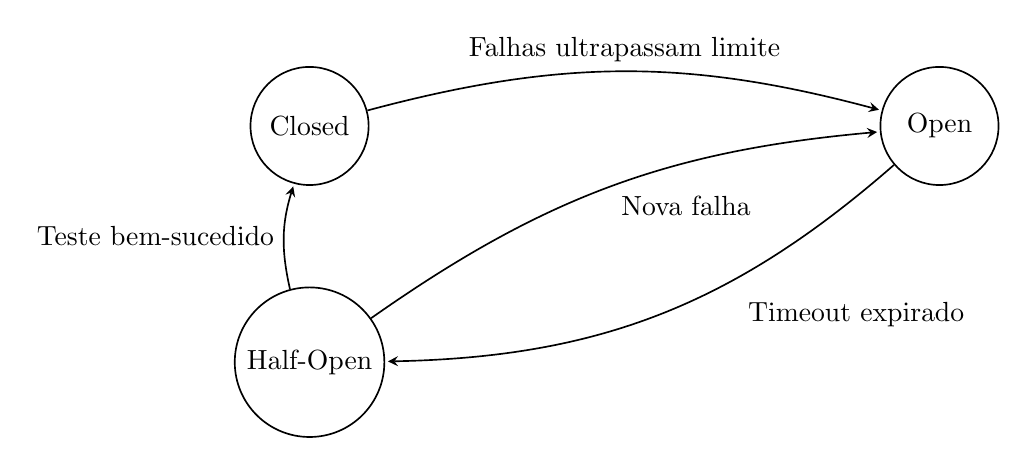
\begin{tikzpicture}[
    ->, >=stealth, shorten >=1pt, auto, node distance=3.5cm, semithick,
    state/.style={circle, draw, minimum size=1.5cm}
  ]
  \node[state] (closed) {Closed};
  \node[state, right of=closed, node distance=8cm] (open) {Open};
  \node[state, below of=closed, node distance=3cm] (halfopen) {Half-Open};
  
  \draw[->] (closed) edge[bend left=15] node[above] {Falhas ultrapassam limite} (open);
  \draw[->] (open) edge[bend left=20] node[right, xshift=10mm] {Timeout expirado} (halfopen);
  \draw[->] (halfopen) edge[bend left=15] node[left] {Teste bem-sucedido} (closed);
  \draw[->] (halfopen) edge[bend left=15] node[below right] {Nova falha} (open);
\end{tikzpicture}
\vspace{1.0cm}
\caption{Modelo de estados do padrão Circuit Breaker}
\label{fig:tikz-circuit-breaker}
\end{figure}

Quando ocorre uma falha e o circuito se abre, o parâmetro \textit{timeout} define o período de espera antes de permitir novas tentativas. Após esse período, o estado \textit{Half-Open} libera requisições de teste: se bem-sucedidas, o circuito fecha novamente; se falharem, o circuito permanece aberto para proteger o serviço de uma nova sobrecarga.

A configuração desses limites e tempos de espera é delicada: valores muito baixos podem cortar requisições antes do necessário, enquanto valores altos demais podem manter um serviço falho ativo por muito tempo. Assim como nos padrões \textit{Retry} e \textit{Timeout}, recomenda-se iniciar com valores razoáveis e ajustá-los com base na observabilidade e nas métricas reais do sistema \citep{Newman:15:MS}.

\subsection{Timeout}
O padrão \textit{Timeout} constitui uma estratégia fundamental para reforçar a resiliência de sistemas modernos \citep{kostenko2023antifragile}. Nesse contexto, o \textit{timeout} define o período máximo de espera do microserviço solicitante pela resposta do microserviço requisitado. Se a resposta não chegar dentro desse intervalo, o serviço requisitado é considerado indisponível ou falho \citep{alashqar2022microservices}.

Além disso, a adoção de \textit{timeouts} adequados promove o isolamento de falhas, de forma que possíveis problemas em outros sistemas, subsistemas ou dispositivos não precisem necessariamente se propagar e afetar todo o ambiente. Quando o \textit{timeout} é configurado de maneira apropriada, falhas são isoladas; um problema em outro sistema não precisa, obrigatoriamente, tornar-se o seu problema. \citep{nygard2018release}

Conexões em redes instáveis podem resultar em falhas e lentidão, afetando operações síncronas e, em alguns casos, levando a \textit{deadlocks} — situações em que dois ou mais processos ou \textit{threads} ficam bloqueados esperando recursos indefinidamente \citep{troubitsyna2019}. Para prevenir esses problemas, mecanismos de \textit{timeout} delimitam o período máximo de espera por uma resposta. Sem tais mecanismos, um serviço corre o risco de aguardar indefinidamente \citep{kostenko2023antifragile}.

Conforme ilustra a Figura \ref{fig:interaction-timeout-pattern}, o \textit{Serviço Consumidor} inicia uma contagem de tempo configurada ao enviar a requisição para o \textit{Serviço Provedor}. Se não houver resposta dentro do intervalo estipulado, o mecanismo de \textit{timeout} é acionado, encerrando a espera e reportando uma falha temporária. Isso evita que o consumidor permaneça indefinidamente bloqueado na expectativa de uma resposta que talvez nunca chegue.

\begin{figure}[H] \centering \includegraphics[width=0.5\linewidth]{imagens/interaction-timeout-pattern.png} \caption{Exemplo de Interação do Padrão Timeout \citep{troubitsyna2019}} \label{fig:interaction-timeout-pattern} \end{figure}

É comum também que \textit{timeouts} sejam aplicados em conjunto com novas tentativas de execução (\textit{retries}). O software busca repetir as operações que excederam o tempo limite, proporcionando mais chances de sucesso em condições de rede instáveis \citep{nygard2018release}.

Em aplicações que recebem muitas requisições simultâneas, o uso do padrão \textit{Timeout} pode dificultar o processamento, pois algumas \textit{threads} podem ficar bloqueadas. Além disso, definir um valor de tempo limite apropriado para cada tipo de serviço dependente tende a tornar o sistema mais complexo, já que cada serviço pode exigir configurações específicas \citep{kostenko2023antifragile}.

\subsection{Bulkhead}

Imagine um navio cruzando o oceano. Para proteger a embarcação de um possível naufrágio, engenheiros navais projetaram compartimentos estanques — chamados \textit{bulkheads} — que isolam partes do casco. Assim, mesmo que ocorra uma ruptura e a água invada um compartimento, os demais permanecem intactos, evitando que o dano se espalhe e leve toda a embarcação ao fundo.

Inspirado nessa estratégia de contenção, o padrão \textit{Bulkhead} aplica o mesmo princípio aos sistemas de software: segmentar e isolar recursos críticos para impedir que falhas em uma parte comprometam toda a aplicação \citep{nygard2018release}. A ideia é particionar o ambiente em segmentos autônomos, de modo que cada um possa falhar ou ser sobrecarregado sem arrastar o restante consigo.

No contexto de aplicações modernas, o padrão \textit{Bulkhead} é fundamental para evitar sobrecargas quando diversos serviços ou módulos são executados simultaneamente. Ele promove a criação de “compartimentos” de recursos — como conexões, memória ou threads — para cada serviço, reduzindo a possibilidade de um pico de tráfego ou uma falha em um serviço afetar toda a operação \citep{kostenko2023antifragile}. Isso envolve, por exemplo, a utilização de \textit{pools} de conexões, que atuam como reservatórios compartilhados e configuráveis para gerenciar de forma eficiente o uso de conexões com bancos de dados. A separação desses \textit{pools} por serviço reduz o risco de um serviço monopolizar todas as conexões disponíveis, comprometendo o desempenho de outros módulos \citep{Sobri2022} 

\begin{figure}[H]
\centering
\includegraphics[width=0.8\linewidth]{imagens/bulkhead-pattern-diagram.png}
\caption{Exemplo de Bulkhead \citep{alashqar2022microservices}}
\label{fig:bulkhead-pattern-diagram}
\end{figure}

À esquerda, vemos um único \textit{pool} de conexões compartilhado, no qual dois sistemas legados — Sistema Legado 1 e Sistema Legado 2 — competem pelos mesmos recursos. Nesse cenário, uma falha ou lentidão em um dos sistemas pode consumir todas as conexões disponíveis, impactando diretamente o outro sistema.

À direita, em contrapartida, o padrão \textit{Bulkhead} cria divisórias entre os sistemas, alocando \textit{pools} de conexões separadas. Dessa forma, mesmo que o Sistema Legado 1 enfrente problemas, o Sistema Legado 2 mantém acesso aos seus próprios recursos, permanecendo isolado das consequências do incidente.

Embora eficaz, a aplicação do \textit{Bulkhead} apresenta desafios relacionados à otimização de desempenho e ao equilíbrio entre segmentação e aproveitamento de recursos. Isso envolve analisar e ajustar múltiplas variáveis interdependentes, como o número de instâncias, a quantidade de threads e a memória disponível, sempre considerando as necessidades e restrições de cada serviço \citep{nygard2018release}.

\subsection{Fallback}
Fallbacks são mecanismos acionados quando um serviço remoto apresenta falhas ou está indisponível, direcionando a busca de informações para um serviço alternativo que esteja funcionando adequadamente \citep{Meiklejohn2024}.

Em vez de retornar uma exceção diretamente ao usuário quando algo dá errado, o padrão fallback recorre a ações alternativas, como buscar dados em uma fonte secundária ou enfileirar a solicitação para processamento futuro. Dessa forma, o usuário não recebe um erro imediato, mas pode ser informado de que sua solicitação será atendida posteriormente, garantindo uma experiência mais fluida e confiável \citep{huaylupo2021spring}.

Por exemplo, em um sistema de monitoramento climático, ao solicitar dados meteorológicos, o sistema inicialmente tenta recuperar as informações de uma API principal. Caso essa fonte falhe, o padrão fallback pode redirecionar a consulta para uma base de dados secundária, como registros históricos. Se nenhuma dessas alternativas estiver disponível, a solicitação é enfileirada, e o usuário é notificado de que os dados serão fornecidos assim que possível.

O padrão fallback pode ser arriscado em situações em que a segurança do sistema depende de respostas críticas, como na verificação de fraudes, podendo levar à aprovação de transações fraudulentas.

\section{Cache}

O \textit{cache} é um mecanismo de armazenamento baseado no modelo \textit{key-value}, que mantém dados em memória sem a necessidade de gravação permanente em arquivos. Esse método reduz a quantidade de leituras e escritas realizadas diretamente no disco, proporcionando um desempenho muito superior ao aproveitar a velocidade da memória \textit{RAM} \citep{falkevych2023}.

Uma das soluções mais populares para implementar \textit{cache} em aplicações \textit{web} é o \textit{Remote Dictionary Server} (\textit{Redis}) . O \textit{Redis} é um banco de dados que funciona inteiramente em memória e adota o modelo \textit{key-value} para armazenamento. Além de sua velocidade e simplicidade, destaca-se por oferecer mecanismos avançados de persistência e suporte a diversas estruturas de dados, o que o torna especialmente útil em sistemas distribuídos que requerem alta disponibilidade \citep{Kanthed2023}.

A Figura~\ref{fig:cache-aside} ilustra o funcionamento do \textit{cache} em um cenário onde o \textit{Redis} atua como intermediário entre o usuário e o banco de dados principal. Esse processo ocorre em quatro etapas principais:

\begin{figure}[H]
\centering
\includegraphics[width=0.8\linewidth]{imagens/redis-work.png}
\caption{Fluxo de funcionamento do \textit{Redis} como camada de \textit{cache}, intermediando requisições entre o usuário e o banco de dados.}
\label{fig:cache-aside}
\end{figure}

Nesse cenário, quando o usuário faz uma solicitação de dados, o sistema primeiro consulta o \textit{Redis} para verificar se a informação já está armazenada em memória. Caso os dados estejam disponíveis, o \textit{Redis} responde diretamente ao usuário, reduzindo a latência e poupando recursos do banco de dados. Entretanto, se o \textit{cache} não contiver a informação — situação conhecida como \textit{cache vazio} —, o sistema encaminha a requisição ao banco de dados principal para obter a resposta. Em seguida, além de fornecer a resposta ao usuário, o sistema armazena esses dados no \textit{Redis}, de modo que consultas futuras sejam atendidas diretamente pela camada de \textit{cache}.

Esse modelo, chamado \textit{Cache-Aside} (ou \textit{Lazy Loading}), permite que as informações mais relevantes sejam mantidas em memória, otimizando o tempo de resposta sem comprometer a consistência dos dados \citep{pamula2014}. Apesar de todos os benefícios proporcionados por esse padrão, é essencial que a configuração e o gerenciamento do \textit{cache} sejam realizados de maneira criteriosa, para evitar problemas como o \textit{cache stampede} — ou \textit{dog-piling} —, em que múltiplas requisições simultâneas tentam acessar ou atualizar um dado expirado, sobrecarregando o banco de dados \citep{falkevych2023, vattani2015}. Dessa forma, o uso adequado do \textit{Redis} como camada de \textit{cache} é um fator determinante para garantir alta performance e escalabilidade em sistemas modernos.

\section{Discussão}

A análise dos padrões arquiteturais e tecnologias apresentadas revela um ecossistema interdependente, no qual a resiliência, escalabilidade e eficiência de sistemas distribuídos dependem da combinação estratégica de múltiplas abordagens.

\begin{table}[H]
\centering
\renewcommand{\arraystretch}{1.5}
\setlength{\tabcolsep}{8pt} 
\begin{tabular}{|l|p{5cm}|p{5cm}|}
\hline
\rowcolor[HTML]{EFEFEF} \textbf{Padrão/Mecanismo} & \textbf{Vantagens} & \textbf{Desvantagens} \\ \hline
\textbf{Retry} & 
Permite novas tentativas em falhas transitórias, aumentando a resiliência. & 
Pode causar sobrecarga ou latência se mal configurado. \\ \hline
\textbf{Circuit Breaker} & 
Protege o sistema de sobrecarga ao isolar falhas. & 
Difícil de configurar os limites adequados. \\ \hline
\textbf{Timeout} & 
Evita bloqueios indefinidos e isola falhas. & 
Complexidade em determinar tempos limites ideais. \\ \hline
\textbf{Bulkhead} & 
Isola recursos, prevenindo que a sobrecarga de um serviço afete outros. & 
Requer particionamento cuidadoso dos recursos. \\ \hline
\textbf{Fallback} & 
Oferece alternativas em caso de falhas, garantindo continuidade. & 
Pode comprometer segurança em cenários críticos. \\ \hline
\textbf{Cache} & 
Reduz a latência e melhora o desempenho ao evitar consultas repetitivas ao banco de dados. & 
Risco de inconsistência nos dados armazenados e problemas como \textit{cache stampede}. \\ \hline
\textbf{Load Balancer} & 
Distribui carga entre servidores, otimizando o uso de recursos e aumentando disponibilidade. & 
Pode gerar distribuição desigual se não configurado corretamente, além de desafios em persistência de sessão. \\ \hline
\end{tabular}
\caption{Comparação entre padrões arquiteturais e mecanismos de otimização}
\label{tab:comparativo-padroes}
\end{table}

Embora a Tabela~\ref{tab:comparativo-padroes} sintetize as vantagens e desafios de cada solução, a real efetividade desses padrões só emerge quando contextualizada em cenários práticos, considerando sinergias entre eles, práticas de desenvolvimento e o ambiente operacional de cada sistema.

Em sistemas distribuídos, falhas são inevitáveis e podem ocorrer em diferentes níveis — desde a comunicação entre microsserviços até a sobrecarga de servidores ou a indisponibilidade temporária de componentes críticos. Por isso, a escolha entre esses padrões não é excludente, mas sim complementar, pois cada abordagem atua de forma distinta, tratando problemas específicos sem necessariamente substituir as demais.

Por exemplo, em ambientes de alta demanda e acesso concorrente, o padrão de \textit{cache} surge como solução para reduzir a latência e aliviar a carga do banco de dados, como observado no uso do \textit{Redis}, que armazena dados em memória para agilizar o atendimento de requisições subsequentes. Esse mecanismo, ao atuar como intermediário entre o usuário e o banco de dados, colabora para a resiliência ao mitigar gargalos de leitura em cenários críticos (\citeauthor{Kanthed2023}, \citeyear{Kanthed2023}). Entretanto, esses mesmos recursos de cache introduzem desafios adicionais, como riscos de inconsistência e fenômenos de \textit{cache stampede}, que surgem em cenários de grande volume de requisições concorrentes \citep{falkevych2023}.

Além disso, como indicam as observações do texto de referência, padrões como \textit{Retry}, \textit{Circuit Breaker} e \textit{Fallback} atuam de forma complementar para lidar com diferentes tipos de falhas. O \textit{Retry} permite novas tentativas de comunicação em falhas transitórias, mas pode sobrecarregar o sistema caso não seja limitado adequadamente. Nesse ponto, a integração com \textit{Circuit Breaker} se mostra essencial, pois ele bloqueia temporariamente chamadas que excedam um limiar de falhas, prevenindo sobrecarga e evitando que um serviço instável agrave a situação. Essa combinação inteligente entre padrões fortalece a resiliência e a eficiência do sistema.

No contexto do modelo de maturidade proposto por esta pesquisa, esses resultados reforçam que a resiliência em sistemas distribuídos não depende de um único padrão ou ferramenta, mas sim de um ecossistema que integra práticas de monitoramento, adaptação e aprendizado. O ajuste contínuo de parâmetros, como tempos de \textit{timeout} e limites de falha do \textit{Circuit Breaker}, aliado a práticas de observabilidade como \textit{tracing} e análise de métricas, confirma a relevância de alinhar a arquitetura técnica com as necessidades do domínio e as características dinâmicas do ambiente \citep{Newman:15:MS, kostenko2023antifragile}.

Em suma, a maturidade em resiliência, tema central desta pesquisa, não se alcança pela simples aplicação de padrões isolados, mas sim pela capacidade de integrá-los de forma coesa, considerando seus \textit{trade-offs} (as compensações necessárias para equilibrar vantagens e desvantagens em cada decisão arquitetural) e ajustando-os às necessidades específicas de cada serviço. Essa integração, combinada com uma cultura organizacional de aprendizado e adaptação, garante que tecnologias como \textit{cache Redis} e \textit{Bulkhead} atuem como elementos de um ecossistema resiliente, preparado para lidar com falhas inevitáveis.
